\documentclass[12pt]{article}
\usepackage[utf8]{inputenc}
\usepackage{latexsym,amssymb,amsmath} % for \Box, \mathbb, split, etc.
% \usepackage[]{showkeys} % shows label names
%\usepackage{cite} % sorts citation numbers appropriately
\usepackage{path}
\usepackage{url}
\usepackage{verbatim}
\usepackage[pdftex]{graphicx}
\usepackage{epstopdf}

%\usepackage[lf]{venturis}

\usepackage{booktabs}
\usepackage{array}
\newcolumntype{L}[1]{>{\raggedright\let\newline\\\arraybackslash\hspace{0pt}}m{#1}}
\newcolumntype{C}[1]{>{\centering\let\newline\\\arraybackslash\hspace{0pt}}m{#1}}
\newcolumntype{R}[1]{>{\raggedleft\let\newline\\\arraybackslash\hspace{0pt}}m{#1}}

\usepackage{subcaption}
\usepackage{pdflscape}
\usepackage{rotating}
\usepackage{cite}

\usepackage[inline]{enumitem}
\newlist{listahorizontal}{enumerate*}{1}
\setlist[listahorizontal]{label=(\alph*)}

% horizontal margins: 1.0 + 6.5 + 1.0 = 8.5
\setlength{\oddsidemargin}{0.0in}
\setlength{\textwidth}{6.5in}
% vertical margins: 1.0 + 9.0 + 1.0 = 11.0
\setlength{\topmargin}{0.0in}
\setlength{\headheight}{12pt}
\setlength{\headsep}{13pt}
\setlength{\textheight}{625pt}
\setlength{\footskip}{24pt}

\renewcommand{\textfraction}{0.10}
\renewcommand{\topfraction}{0.85}
\renewcommand{\bottomfraction}{0.85}
\renewcommand{\floatpagefraction}{0.90}
\renewcommand{\baselinestretch}{1.2}

\makeatletter
\setlength{\arraycolsep}{2\p@} % make spaces around "=" in eqnarray smaller
\makeatother

% change equation, table, figure numbers to be counted inside a section:
\numberwithin{equation}{section}
\numberwithin{table}{section}
\numberwithin{figure}{section}

% begin of personal macros
\newcommand{\half}{{\textstyle \frac{1}{2}}}
\newcommand{\eps}{\varepsilon}
\newcommand{\myth}{\vartheta}
\newcommand{\myphi}{\varphi}

\newcommand{\IN}{\mathbb{N}}
\newcommand{\IZ}{\mathbb{Z}}
\newcommand{\IQ}{\mathbb{Q}}
\newcommand{\IR}{\mathbb{R}}
\newcommand{\IC}{\mathbb{C}}
\newcommand{\Real}[1]{\mathrm{Re}\left({#1}\right)}
\newcommand{\Imag}[1]{\mathrm{Im}\left({#1}\right)}

\newcommand{\norm}[2]{\|{#1}\|_{{}_{#2}}}
\newcommand{\abs}[1]{\left|{#1}\right|}
\newcommand{\ip}[2]{\left\langle {#1}, {#2} \right\rangle}
\newcommand{\der}[2]{\frac{\partial {#1}}{\partial {#2}}}
\newcommand{\dder}[2]{\frac{\partial^2 {#1}}{\partial {#2}^2}}

\newcommand{\nn}{\mathbf{n}}
\newcommand{\xx}{\mathbf{x}}
\newcommand{\uu}{\mathbf{u}}

\newcommand{\junk}[1]{{}}

% set two lengths for the includegraphics commands used to import the plots:
\newlength{\fwtwo} \setlength{\fwtwo}{0.45\textwidth}
% end of personal macros
\graphicspath{ {../../../resources/images/vectors/}{../../../resources/images/bits/} }

\begin{document}
%\DeclareGraphicsExtensions{.jpg}

\begin{center}
\textbf{\Large Smart Usage of Context Information for the Analysis, Design, and Generation of Power-Aware Policies for Mobile Sensing Apps} \\[16pt]


\includegraphics[scale=0.08]{cinvestav2.jpg}

\textbf{Technical Report}\\[6pt]
LTI-TR-2014-07 \\[16pt]

\textbf{Student} Rafael Pérez-Torres \\[6pt]
\textbf{Advisors} César Torres Huitzil Phd, Hiram Galeana Zapién Phd.\\[16pt]

Information Technology Laboratory,\\
CINVESTAV Tamaulipas \\[16pt]

%  gobbert@umbc.edu, \url{www.math.umbc.edu/~gobbert}
\end{center}

\abstract{
This technical report describes the progress and advances developed for the thesis work titled \emph{Smart Usage of Context Information for the Analysis, Design, and Generation of Power-Aware Policies for Mobile Sensing Apps} during the first year of the doctoral program.

In summary, the different efforts during the first year have been focused on producing a solid state of the art revision, as well as on defining the core elements that will power up the methodology for solving the main problem.
}

\subparagraph{Keywords.} mobile sensing apps, energy consumption, context information, policy, smartphone.

\section{Introduction}
\label{sec:introduction}
OK REMEMBER THIS IS TECHNICAL, YOU CAN DESCRIBE AT TECHNICAL DETAIL THE SECTIONS
This technical report describes the progress and advances developed for the thesis work titled \emph{Smart Usage of Context Information for the Analysis, Design, and Generation of Power-Aware Policies for Mobile Sensing Apps} during the first year of the doctoral program.

In summary, the different efforts during the first year have been focused on producing a solid state of the art revision, as well as on defining the core elements that will power up the methodology for solving the main problem.


In order to ease the comprehension for the reader, this report has been structured as a self-contained document, briefly addressing the scientific context of the research, describing the hypothesis, problem statement and objectives.
This technical report is structured as follows.
Section~\ref{sub:research-context} presents a brief review of the context of the research.
Section~\ref{sec:state-of-art} is prepared as for describing the study performed on state-of-art techniques, covering a taxonomy of previous solutions and a framework for their analysis.
Section C is aimed at describing the advances produced on our proposed solution, including the insights for achieving learning from user and a general overview of the mechanisms for achieving sensor usage adaptations.
Section D addresses some FUTURE WORK!
Section E summarizes the scientific products prepared during this first year of work.
Finally, Section F present the conclusions of this report.










% *************************************
% *************************************
% ****** 1. Research description ******
% *************************************
% *************************************
\section{Research description}
\label{sub:research-context}
\emph{This section is aimed at giving an overall description of the context of the research, in order to ease the comprehension of the reader and producing a self-conteined document.}


%\subsection{Motivation of this research}
The popularity of smartphones is a remarkable instance of the adoption of technology by society.
According to the Ericsson Mobility report~\cite{Ericsson2015} there were 3,400 million of smartphone subscriptions and 250 million of mobile PCs, tablets and mobile router subscriptions in the 2015.
The presence of smartphones is drastically changing our daily lives by providing an increasingly powerful set of tools as a result of significant advances in the field.
% It is expected to have 6,400 million and 350 million of subscriptions, respectively, by the end of the 2021.
The capabilities and platform complexity of smartphones are continuously improving, becoming truly system-on-chip (SoC) devices able to adapt their operation over three distinguishing dimensions, namely communication, sensing, and computation, as conceptually shown in Figure~\ref{fig:smartphone-dimensions}.
The advances on these dimensions have enabled the \emph{context-awareness}~\footnote{For the sake of clarity, we stick to the definition of \emph{context} proposed by \cite{Chen2000}, as the set of environmental states and settings that either determines the application’s behavior or in which an application event occurs and is interesting to the user.} paradigm in mobile and pervasive computing, opening the path for a myriad of applications and services.
Particularly in the sensing dimension, modern smartphones include a set of low cost and powerful embedded sensors such as accelerometer, digital compass, gyroscope, GPS receiver, microphone, and camera, among others, providing them with rich capabilities for creating mobile sensing applications at different spatial and temporal scales~\cite{Lane2010,Campbell2012,Kjaergaard2012} and with different levels of accuracy and energy costs.
For this class of applications, the core requirements are the background and continuous sensors' data acquisition, as well as the associated on-device computations for extracting useful information for the user~\cite{Lane2010,Ra2012}.
As user interaction can be required for collecting data, two sensing paradigms can be implemented~\cite{Lane2010}.
The \emph{opportunistic paradigm} tries to determine the most appropriate moment for automatically collecting data from sensors without human participation at all.
On the other hand, the \emph{participatory paradigm} leverages user's abilities requiring his/her participation to describe data and choose the moment for collecting them.
Given its autonomy, the opportunistic paradigm represents the preferable choice for continuous mobile sensing.

\begin{figure}[t]
  \centering
  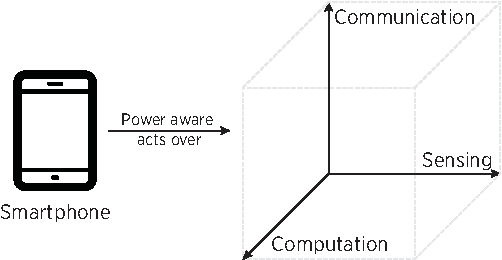
\includegraphics[scale=0.75]{smartphone-dimensions}
  \caption{The communication, computation, and sensing features offered by smartphones represent the main dimensions where the functionality of these devices relies on.}
  \label{fig:smartphone-dimensions}
\end{figure}


\subsection{Smartphone-based sensing characteristics}
Regardless of the sensing paradigm, the internal operation of mobile sensing applications commonly involves a set of stages that describe the closed loop shown in Figure~\ref{fig:stages-of-power-aware-mobile-sensing}, consisting in:
\begin{listahorizontal}
  \item \emph{Sensor reading} that involves selecting, configuring, and requesting data to sensors,
  \item An \emph{optional preprocessing} for discarding uninteresting data like outliers or reducing noise,
  \item \emph{Feature extraction} for obtaining features, i.e., more computationally efficient representations of data,
  \item \emph{Classification} of extracted features into classes of special interest, for example human activity aspects that might feed machine learning strategies, and
  \item \emph{Post-processing} for offering feedback to user, launching network communication, triggering another sensing-classification chain with the outcome of classification acting as feedback information for a more precise operation of sensors, or for performing further processing.
\end{listahorizontal}
At each stage, the level of context-awareness of the mobile platform is increased, requiring specific algorithmic solutions to perform the above described functions.
The design of such solutions is not straightforward, as there are a number of factors that impact the operation of each stage.
This is the case of the dynamics of user's context which depends on changes produced in the environment, the existing constraints in mobile platforms, and the privacy concerns of personal data manipulation that, as a whole, compromise the sensor readings, classification and post-processing of data.
Similarly, the implementation of these applications is hindered by priorities and additional requirements like the latency at which a context change is detected, the accuracy of the inferred context, and the implicit rational usage of energy resources.
\begin{figure*}[t]
    \centering
    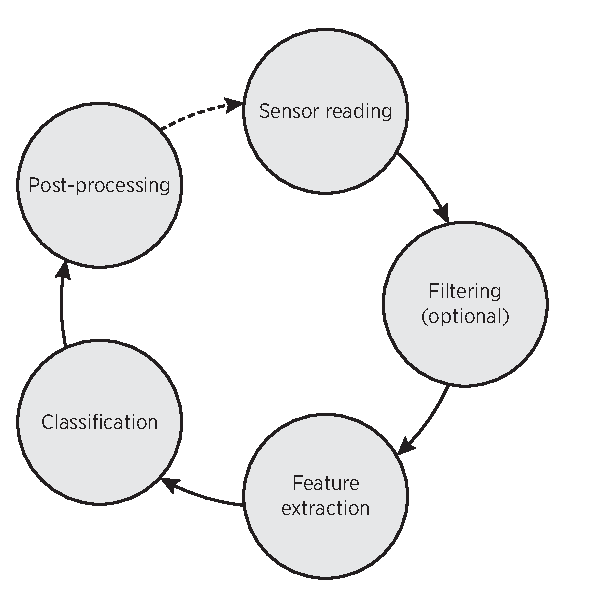
\includegraphics[width=\textwidth]{msa-stages}
    \caption{The different stages of mobile sensing applications produce output, shown in the lower gray rounded boxes, whose level of information is increasing at each stage. The post-processing stage might launch a new sensor reading chain as shown by the top dashed line.}
    \label{fig:stages-of-power-aware-mobile-sensing}
\end{figure*}

Despite the fact there is a common understanding of how to deploy the aforementioned stages in mobile sensing applications, the support for continuous sensing is still an open research problem due to the power demands of long-term sensing and the inherent resource-constrained characteristics of mobile devices.
Although modern smartphones feature increasing computing power, memory and longer battery life, the requirements of complex mobile sensing applications represent a great challenge for mobile platforms, especially to the battery consumption, whose typical capacity is on the order of thousands of mAh, growing only 5-10\% each year~\cite{Ma2012,Evarts2015}. 
This growing rate is not at the same pace than the advances in hardware and software components of mobile platforms, which in every new generation of mobile devices impose an ever growing energy demand.

At the same time, it is important to note that since their initial conception, mobile platforms described a layered architecture with a clear focus on managing the heavy interaction with user.
because of this, the support for background running processes and for exploiting the power management capabilities existing at hardware level of sensors was discarded, leaving out the power-efficiency of the sensing dimension~\cite{Priyantha2011}.
As a consequence, efficient implementations of power-aware mechanisms that do not jeopardize the accuracy requirements of mobile sensing applications still remain an open challenge, which is augmented by the computational and power constraints of mobile devices, as well as the long-term and near real-time requirements of these applications.


\subsection{Hypothesis} 
\label{sub:hypothesis}
As previously described, long-time operation of mobile sensing applications remains as an open challenge, due to the inherent trade-off between the energy consumed when accessing to sensors and the accuracy of the activity being tracked.
In simpler terms, the more accuracy obtained when accessing sensors with high frequency, the higher energy consumption.
Nonetheless, this research work considers that the dynamics of context information inferred from sensors data is of remarkable value for adapting sensory operations and producing power savings.
Thus, the hypothesis pursued in this work states that \emph{intelligent policies produced through context information built from sensors data can be employed to reduce the energy consumption in a mobile device when performing continuous sensor readings}.

In a deeper description, a smart policy is a special rule that defines how sensors should be accessed in order to reduce the energy consumption and achieve mobile app requirements.
This research work aims to employ data coming from GPS and inertial sensors in order to obtain context information in terms of mobility patterns, useful to reduce the energy consumption generated by LBS's~\footnote{LBS, Location Based Service.}.


\subsection{Problem statement} 
\label{sub:problem_statement}
In order to prove the aforementioned hypothesis, this research work identifies the existence of two interrelated problems, which are described as follows.
The first one is depicted as a \emph{pattern identification problem} and is focused on detecting changes in the mobility pattern of user from sensors data.
Such pattern represents the context information that is helpful to add \emph{smartness} to the policies that adapt sensory operations.

Formally:
\label{ssub:pattern_identification}
Given a set $V = \left\{v_{1}, v_{2}, \dotsc, v_{n}\right\}$ of data values read from sensor $S$ in the time interval $T = [t_{1}, t_{2}]$, find the behavior pattern $Pattern_{S}$ that represents the activity of user.

\begin{equation}
  PatternIdentifier( V ) \longrightarrow{} Pattern_{S} \in Patterns
\end{equation}

Where $Patterns$ is a set of patterns that represent an interesting state in the user mobility data, namely $\left\{no\_movement, walking, running, vehicle\_transportation\right\}$.

On the other hand, the \emph{policy generation problem} is related to the selection and configuration of proper sensors for keeping the user location tracking, while at the same time reducing energy consumption.
For this process, it is also important to consider the level of the smartphone's battery and the accuracy requested by the mobile application.

Formally:
Given the detected pattern $Pattern_{S}$ in data from sensor $S$, parameters for assigning weight to energy $eh$, and physical constraints status $pc$ of a mobile device, find a policy to adapt the duty cycle of sensors.

\begin{equation}
  PolicyGeneration( Pattern_{S}, eh, pc ) \longrightarrow{} DutyCycle_{S}
\end{equation}


\subsection{Objectives} 
\label{sub:objectives}

\subsubsection*{Main objective}
\label{ssub:main_objective}
To reduce energy consumption in the mobile sensing apps, which perform continuous sensor readings, through self-adapting power-aware policies generated from context information obtained from sensors data.

\subsubsection*{Particular objectives} 
\label{ssub:particular_objectives}
\begin{itemize}
  \item To identify mobility patterns from context information obtained from an inertial sensor (accelerometer) and location providers (GPS, WPS).
  \item To generate policies for a self-adapting sensors' usage from identified mobility patterns, accuracy and energy requirements of mobile application, and status of mobile device's constraints. 
  \item To ease the development of mobile sensing applications that require user location tracking, i.e., LBS, isolating the complexity of sensors' access and the associated efficient energy management.
\end{itemize}


\subsection{Contributions} 
\label{sub:contributions}

\begin{itemize}
  \item A mechanism for detecting mobility patterns from the data read by sensors of mobile devices (especifically GPS and accelerometer).
  \item A mechanism for generating policies for accessing sensors.
  Such mechanism employs application requirements (energy and precision hints), level of mobile device constraints, and user's context information (using the pattern detected by previous mechanism).
  The produced policies will allow to perform a smarter usage of smartphone's sensing infrastructure in continuous sensor readings, reducing the energy consumption.
  \item A middleware that implements the previously described mechanisms, easing the development of mobile sensing applications.
\end{itemize}










% *************************************
% *************************************
% ****** 2. State of art related ******
% *************************************
% *************************************
\section{State of art analysis}
\label{sec:state-of-art}
Research on power consumption of mobile devices started since their conception and introduction to the market, and has produced several power management strategies that show an evolution on their complexity and flexibility.
Early techniques consisted on generic mechanisms for accessing platform components, mostly at hardware level, like adapting their voltage and frequency of operation, as well as modifying their active power mode~\cite{Mayo2003,Lorch1998,Benini2000}.
Current strategies are focused in specific design issues of particular sensors, tasks, and scenarios where both hardware and software scale their features and energy usage according to changes in the mobile platform workload~\cite{Lane2010,Hoseini-Tabatabaei2013}.
Intuitively, if there are no hard power consumption constraints, the software stack can use hardware components at maximum performance.
On the other hand, the mobile platform must react accordingly and modify the hardware usage by employing a set of policies that helps to reduce energy consumption and still achieve the accuracy and performance requirements of mobile applications.
Leveraging on context information plays a key role to optimize the \emph{sensor reading} stage (represented in Figure~\ref{fig:stages-of-power-aware-mobile-sensing}), reducing the number of sensor invocations, and producing such smart and dynamic adaptation in the sensing dimension.
On the other hand, ignoring any source of context information at the sensor reading stage will avoid dynamic adaptations, leading to a fixed hardware usage and neglecting power savings.
As a result, there is an inherent power consumption-accuracy trade-off when accessing and consuming sensor data~\cite{Sim2014,Rachuri2012}.

% In contrast, a context-agnostic scheme (that does not use context information on the sensing stage) would omit such adaptation and discard power optimizations, as shown by the upper line in Figure~\ref{fig:comparison-agnostic-aware-mobile-platform}.
% As illustrated conceptually by the plot shown in Figure~\ref{fig:comparison-agnostic-aware-mobile-platform}, leveraging on context information plays a key role to optimize the \emph{sensor reading} stage (represented in Figure~\ref{fig:stages-of-power-aware-mobile-sensing}), to reduce the number of sensor invocations, and to produce a smart and dynamic hardware usage adaptation.
% In contrast, a context-agnostic scheme (that does not use context information on the sensing stage) would omit such adaptation and discard power optimizations, as shown by the upper line in Figure~\ref{fig:comparison-agnostic-aware-mobile-platform}.
\begin{figure*}[t]
  \centering
  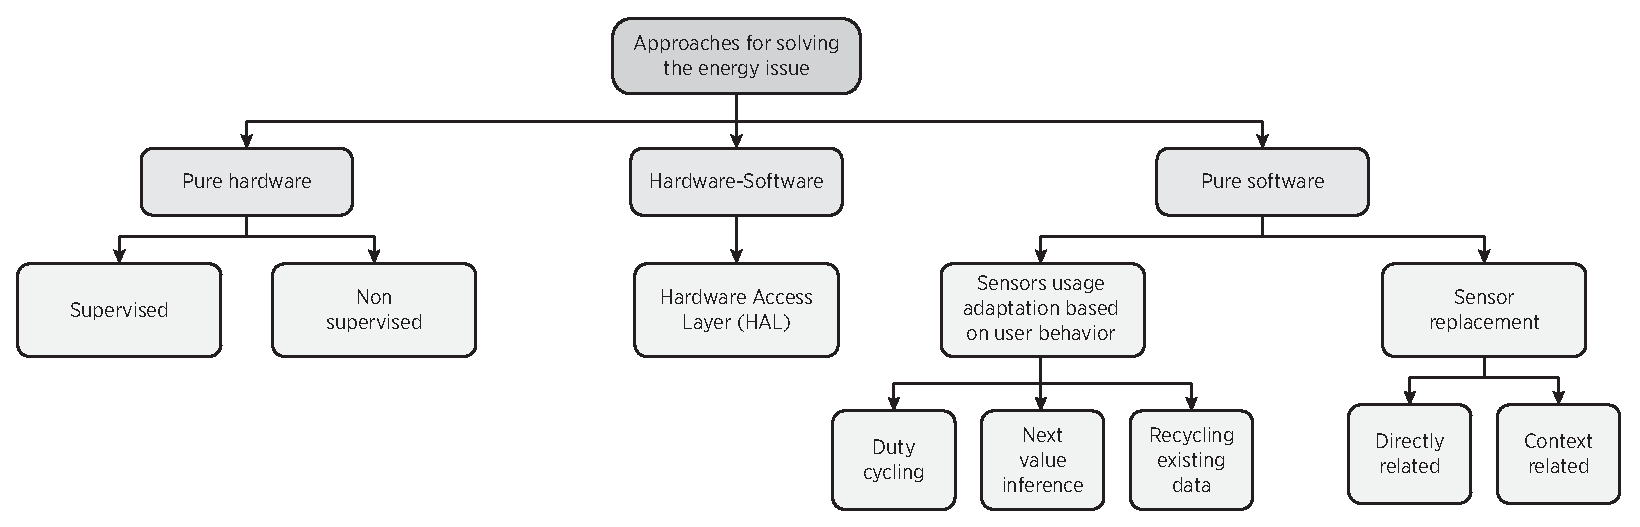
\includegraphics[width=\textwidth]{approaches-taxonomy}
  \caption{The taxonomy of solutions for power-aware smartphone sensing is divided into three categories: pure hardware, hardware-software and pure software.}
  \label{fig:taxonomy-approaches}
\end{figure*}

Power-aware sensing refers to a set of techniques and methodologies aimed at continuously monitoring sensor data over long periods of time under the computing, storage, and power constraints of typical mobile devices.
Roughly speaking, the power-aware sensing is mostly enclosed into the sensor reading stage of mobile sensing applications, abstracting the complexity of sensors management, and delivering collected data while considering the power constraints of these devices. 
It is important to remark that this goal is frequently achieved by executing the rest of the stages internally, in order to identify context information that is useful for feedback purposes and a smarter usage of sensors.
A revision of relevant works in literature reveals three complementary approaches at different level of abstraction of the smartphone device: pure hardware, hardware-software, and pure software approaches, based on the classification of generic power-aware computing techniques described in~\cite{Ranganathan2010}.
The proposed taxonomy, and definition of each of the categories and their specializations, will be described in next subsections.
Figure~\ref{fig:taxonomy-approaches} presents a taxonomy of solutions for power-aware smartphone sensing, with the pure hardware, hardware-software and pure software approaches as the main classes, briefly described in the next paragraphs.
These approaches incorporate policies with embedded algorithms that analyze simple or complex context information for controlling the power consumption, producing \emph{recipes for power-aware sensing} in mobile devices.
It has been identified that the support for these policies at system level of a mobile platform facilitates the analysis, control, and cross-layer coordination and information sharing for reducing the power consumption, which is the reason why power-aware sensing mechanisms should be supported throughout all layers of the mobile platform~\cite{Ranganathan2010}.
Figure~\ref{fig:distribution-approaches} illustrates the distribution of the different approaches across the layers of a mobile platform, highlighting the increasing support in the higher layers for reacting accordingly to the dynamics of context information through more complex and robust machine learning mechanisms.
The distinctive characteristics of the different approaches are as follows:
\begin{figure}[t]
  \centering
  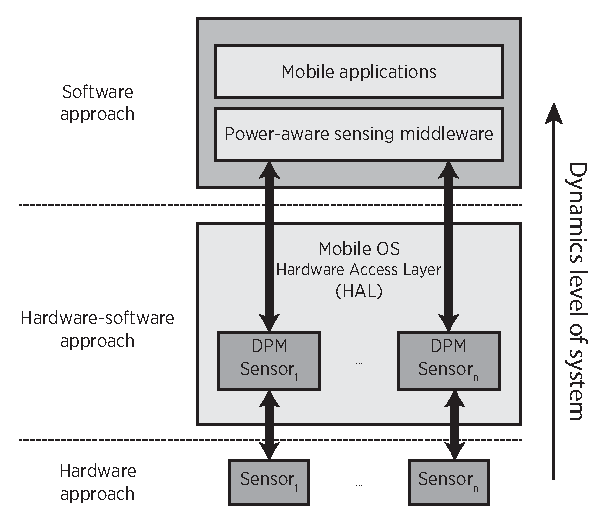
\includegraphics[width=0.5\columnwidth]{approaches-distribution}
  \caption{The approaches distributed across the mobile platform stack are more adaptive to system's dynamics on the higher layers.}
  \label{fig:distribution-approaches}
\end{figure}
\begin{itemize}
  \item The \textbf{pure hardware approach} is the lowest level at which power-aware optimizations could be performed.
  It involves the selection of power-aware sensors and embedded components to deliver physical data to upper layers of mobile platform, as well as the definition of the different power modes of the hardware components through techniques like Dynamic Voltage and Frequency Scaling (DVFS)~\cite{Priyantha2011,Choi2010}.
  Such power modes define a static behavior of hardware components, which can be adapted through hardware control points exported to upper layers, as in~\cite{Priyantha2011,Choudhury2008,Apple2015}.
  \item The \textbf{hardware-software approach} abstracts fine grain details and isolates the usage of hardware components for mobile applications and upper platform layers.
  This isolation is performed by applying system-wide policies that coordinate the operation and interaction of the whole set of sensors according to dynamic changes in their workload and global status of the mobile platform (like battery level).
  The hardware-software approach is aware of the hardware components of the mobile platform, and is able to define DPM mechanisms for turning sensors on and off, and adapt their configuration parameters, as proposed in~\cite{Ra2012,Zhuang2010}.
  \item The \textbf{pure software approach} is aimed at modeling, identifying and even predicting details about context information and its dynamic changes from sensor data, in order to define smart mechanisms for power-aware adaptation of the hardware components usage, like the implementations by~\cite{Chon2014,Yurur2014,MaY2009}.
  Because of the fully context-awareness that this approach achieves, it is able to obtain high levels of flexibility for adaptive management of sensors, and put the context information detected from sensors data at service of the whole mobile platform.
\end{itemize}

% http://bit.ly/1M2sLVr
%\newgeometry{left=1.7cm}
\begin{table*}
    \centering
    \scriptsize{}
    
    %\begin{tabular}{C{0.07\linewidth}C{0.21\linewidth}C{0.28\linewidth}C{0.2\linewidth}C{0.1\linewidth}}
    \begin{tabular}{C{0.09\linewidth}C{0.17\linewidth}C{0.25\linewidth}C{0.18\linewidth}C{0.17\linewidth}}
    \toprule
    \textbf{Year} & \textbf{Name} & \textbf{Mobile platform} & \textbf{Description} & \textbf{Approach} \\
    \midrule
    \cite{Choudhury2008} 2008 & \emph{The Mobile Sensing Platform} & Intel iMote with custom hardware & User motion & Pure hardware \\
    \cmidrule(l){1-5}
    \cite{Priyantha2011} 2011 & \emph{LittleRock} & Not specified & User motion & Pure hardware \\
    \cmidrule(l){1-5}
    \cite{Apple2015} 2013 & \emph{Apple iPhone 5s} & Apple iPhone 5s and newer & User motion & Pure hardware \\
    \cmidrule(l){1-5}
    \cite{Zhuang2010} 2010 & Not given & Android G1 (Android 1.5) & User location & Hardware-Software \\
    \cmidrule(l){1-5}
    \cite{Ra2012} 2012 & Not given & Samsung SGH-i917 (Windows Phone 7.5) & Generic sensors access & Hardware-Software \\
    \cmidrule(l){1-5}
    \cite{Constandache2009} 2009 & \emph{EnLoc} & Nokia N95 (Symbian 60) & User location & Pure software \\
    \cmidrule(l){1-5}
    \cite{Abdesslem2009} 2009 & \emph{SenseLess} & Nokia N95 (Symbian 60) & User location & Pure software \\
    \cmidrule(l){1-5}
    \cite{Wang2009} 2009 & \emph{EEMSS} & Nokia N95 (Symbian 60) & User location, user activity & Pure software \\
    \cmidrule(l){1-5}
    \cite{Kjaergaard2009} 2009 & \emph{EnTracked} & Nokia N95 (Symbian 60) & User location & Pure software \\
    \cmidrule(l){1-5}
    \cite{MaY2009} 2009 & \emph{iLoc} & Simulation & User location & Pure software \\
    \cmidrule(l){1-5}
    \cite{Paek2010} 2010 & \emph{RAPS} & Nokia N95 (Symbian 60) & User location & Pure software \\
    \cmidrule(l){1-5}
    \cite{Kim2010} 2010 & \emph{SensLoc} & Simulation & User location & Pure software \\
    \cmidrule(l){1-5}
    \cite{Perez2010} 2010 & \emph{G-Sense} & Simulation & User location, user activity & Pure software \\
    \cmidrule(l){1-5}
    \cite{Lin2010} 2010 & \emph{A-Loc} & Simulation and Android G1 & User location & Pure software \\
    \cmidrule(l){1-5}
    \cite{Lu2010} 2010 & \emph{Jigsaw} & Nokia N95, Apple iPhone & User location, user activity & Pure software \\
    \cmidrule(l){1-5}
    \cite{Chon2011} 2011 & \emph{SmartDC} & HTC Desire (Android 2.1) & User location & Pure software \\
    \cmidrule(l){1-5}
    \cite{Paek2011} 2011 & \emph{CAPS} & Nexus One (Android 1.5-2.2) & User location & Pure software \\
    \cmidrule(l){1-5}
    \cite{Srinivasan2012} 2012 & Not given & Simulation & User activity & Pure software \\
    \cmidrule(l){1-5}
    \cite{Perez-Torres2012} 2012 & Not given & Samsung Galaxy S (Android 2.3) &  User location & Pure software \\
    \cmidrule(l){1-5}
    \cite{Zhang2013} 2013 & \emph{SensTrack} & Google Nexus S (Android 4.1.4) & User location & Pure software \\
    \cmidrule(l){1-5}
    \cite{Mazilu2013} 2013 & \emph{Not given} & Custom Samsung Galaxy Nexus, and Samsung Galaxy S4 (Android) & User location & Pure software \\
    \cmidrule(l){1-5}
    \cite{Chon2014} 2014 & \emph{FreeTrack} & Smartphone not specified (Android 2.2) & User location & Pure software \\
    \cmidrule(l){1-5}
    \cite{Man2014} 2014 & Not given & Samsung Galaxy III (Android 4.1.4) & User location & Pure software \\
    \cmidrule(l){1-5}
    \cite{Yurur2014} 2014 & Not given & Blackberry Storm II & User activity & Pure software \\
    \cmidrule(l){1-5}
    \cite{Donohoo2014} 2014 & Not given & HTC MyTouch 3G, Google Nexus One, and others (Android) & User location, user activity & Pure software \\
    \cmidrule(l){1-5}
    \cite{AlvarezDeLaConcepcion2014,Morillo2015} 2014 & Not given & Google Nexus One & User activity & Pure software \\
    \cmidrule(l){1-5}
    \cite{Khalifa2015} 2015 & Not given & Simulation (of energy harvesting device) & User activity & Pure software \\
    \bottomrule
    \end{tabular}
    \protect\caption{A set of produced works aimed at solving the power consumption issue in smartphone-based mobile sensing. Most of the solutions follow a pure software approach, given its flexibility and adaptive features.\label{tab:related-work}}
    
\end{table*}
%\restoregeometry


It is important to highlight that although the presented taxonomy allows to classify the power-aware smartphone-based sensing techniques, the relevance of this problem makes that in practice many of the solutions combine different strategies pursuing an integral and better power management.
This is a suggestion of the complexity of the problem itself and an evidence of the evolution and adoption of these complementary techniques.
Furthermore, ideas proved to be working efficiently in software soon or later are implemented directly in hardware to boost efficiency even further. 

Despite the different approaches for achieving power-aware sensing may be applicable to any set of sensors, in practice they have been mainly employed for optimizing power consumption of location providers, like the GPS and Wi-Fi Positioning System (WPS), in continuous Location-based Services (LBS).
The reason behind this trend is twofold.
On one hand, the optimization of energy hungry hardware elements like the GPS and other radio interfaces (i.e., GPRS, Bluetooth, etc.), allows the different power-aware sensing techniques to prove their effectiveness under the most strident conditions in terms of energy consumption than those observed in applications that make use of lower power consumption sensors.
On the other hand, location information in smartphones is required by a wide variety of applications and therefore, the optimization of energy resources of the GPS sensor reading process (which is the core enabler of LBS) is required.
Nonetheless, it is noteworthy that the principles of some of the different proposed solutions can be tailored and implemented in other application niches employing different sensors.

Table~\ref{tab:related-work} summarizes a set of works found in literature aimed at solving the power consumption issue in mobile sensing applications in the context of the presented taxonomy.
As it can be noted, the most common strategy followed in the literature is the pure software approach, due to its flexibility and fine-tuning features, which will be described in next sections of this paper.
Because of the heterogeneity of target features, main purpose, and mobile platforms where the mechanisms proposed in each work were implemented, it is not straightforward to perform a fair comparison among them~\cite{Vallina-Rodriguez2013,Neely2008}.
For example, the solutions may target a different set of sensors or the techniques for analyzing context information produce outputs with different semantic meaning.
Also there is no a clear consensus for measuring the energy benefits of proposed solutions; in this regard two main strategies have been followed.
The first and most common strategy is to perform a comparison in terms of mW between energy consumed by a solution and the mobile platform or a similar approach. 
However, even inside this strategy the implementations are not homogeneous and the proposed solutions employ different methods for measuring energy consumption in mobile devices, namely highly-invasive, moderately-invasive, and non-invasive techniques, as described in~\cite{Abreu2012}.
The second strategy performs the comparison in terms of battery life (e.g., time to drain) because, according to~\cite{Kim2014}, several physical characteristics of batteries impact on their discharging cycle.
The most notorious aspect is that the actual available energy is reduced when the battery discharges, a behavior that is ignored in the energy consumption models included in most of the reviewed solutions.

The next sections of the document present a description of relevant aspects about the different approaches of the proposed taxonomy.
Important concepts about the pure hardware and hardware-software approaches have been already discussed in existing works~\cite{Priyantha2011,Ranganathan2010,Lorch1998,Benini2000}.
Hence, this survey includes a brief description about them, as well as the analysis of associated specializations found in state-of-art works.
Subsequently, a detailed analysis of the features offered by the pure software approach is presented.
This analysis includes its fundamental aspects, its advantages and possibilities when compared against other approaches, as well as the description of its flexibility for modeling and adapting to dynamic changes in context information, which makes it ideal for fitting the system behavior according to user profile.


\subsection{Pure hardware approach}
The fundamental idea behind the pure hardware approach is the selection of power-aware hardware elements for providing physical data to upper layers of the mobile platform, as well as the definition of mechanisms to adapt the hardware input parameters, like DVFS.
These mechanisms allow the creation of control points for manipulating hardware usage, which are known as power modes~\cite{Ranganathan2010,Lorch1998,Benini2000}.
The mobile platform keeps the list of power modes fixed and instruct sensors to work isolated from others.
In this way, the hardware components obey a static behavior defined only through power modes, whose control points are exported to upper layers of the mobile platform.

The set of works under this approach typically involve the design of specific hardware to exploit the aforementioned features.
This design implies the isolation of the components associated with the measurement of physical signals inside a new unit with a dedicated low power processor (LPP).
% This new hardware unit can obtain a substantial reduction in the energy consumption since it is energy aware by design and typically does not imply a modification in the logic of mobile applications.
Since the mobile OS isolates the access to these hardware components, mobile applications remain agnostic about the new hardware unit and can consume its power-aware sensing services without modifying their inner logic.
The basic behavior of this unit requires sensors to report their readings to the embedded LPP, which is capable of executing light preprocessing operations like noise filtering.
While the hardware unit performs the reading and filtering stages, the rest of the smartphone hardware platform is able to reach its sleep mode, producing power savings.
Table~\ref{tab:works-hardware-approach} shows some of the most representative works under the pure hardware approach.
Depending on the ability to process data and discover contextual information autonomously, the pure hardware approach can be implemented in two different ways, namely the \emph{ad-hoc data acquisition} and the \emph{co-processing} variants, as shown in Figure~\ref{fig:taxonomy-approaches}.

\begin{table}[t]
    \centering
    \scriptsize{}
    \begin{tabular}{C{0.25\columnwidth}C{0.2\columnwidth}C{0.4\columnwidth}}
    \toprule
    \textbf{Name} & \textbf{Variant} & \textbf{Sensors involved} \\
    \midrule
    LittleRock \cite{Priyantha2011} & Ad-hoc data acquisition &  Accelerometer, compass, gyroscope \\
    
    Apple iPhone 5s \cite{Apple2015} & Coprocessing & Accelerometer, compass, gyroscope \\

    The Mobile Sensing Platform \cite{Choudhury2008} & Coprocessing & Accelerometer, barometer, compass, humidity, light, microphone, temperature \\
    \bottomrule
    \end{tabular}
    \protect\caption{Representative works under the pure hardware approach. More context-aware features are being deployed directly into hardware components of mobile platforms.\label{tab:works-hardware-approach}}
\end{table}


The \emph{\textbf{ad-hoc data acquisition}} variant is restricted to serve the different mobile application requests for raw sensor data, discarding the analysis and extraction of higher level information.
For instance, \emph{LittleRock}, proposed by Priyantha \emph{et al.}, in~\cite{Priyantha2011}, defines a specific unit with embedded sensors powered directly from battery, allowing the main circuitry of the smartphone to reach the sleep mode while performing sensor readings.
Once a special event defined by a mobile application is detected in data coming from sensors, \emph{LittleRock} is able to wake up the phone for further processing.
\emph{LittleRock} is faster than the phone itself to collect a single sample of data from sensors, due to the complexity of the software stack that smartphone's main processor has to handle.

Besides the raw data delivery, the \emph{\textbf{co-processing}} variant adds support to hardware layers for light data processing and detection of higher level information, producing context-awareness at hardware level with low power consumption.
In this sense, the sensing facilities of the hardware platform are transformed into smart sensors~\cite{Gervais-Ducouret2011}.
The embedded LPP of the sensing unit must be powerful enough to perform such analysis.

Smartphone manufacturers have begun to integrate into the device's hardware full suites of sensing capabilities.
For instance, Apple has implemented a platform re-design of the \emph{iPhone} smartphone, which starting at \emph{5s} version features an isolated sensing unit able to process sensor data and deliver fitness information like the amount of steps and distance covered by user, as well as the type of activity performed, namely, stationary, walking, running, automotive, cycling, and unknown~\cite{Apple2015}.
In addition to this hardware platform update, the Software Development Kit (SDK) of iPhone exposes this functionality through a software Application Programming Interface (API) denominated the \emph{CoreMotion Framework} that enables mobile applications to request and consume the fitness information.
A similar co-processing mechanism is implemented by Choudhury \emph{et al.}, in the \emph{Mobile Sensing Platform} (\emph{MSP})~\cite{Choudhury2008} which employs ad-hoc components for building a custom mobile sensing platform with a LPP able to perform light classification tasks for identifying user activity.

A common aspect taken into account in the design of pure hardware approach solutions is the power consumption - usage generality trade-off that emerges when hardware designers are unable to foresee the needs of any future mobile application and implement power-aware mechanisms to support them directly in the circuits.
Because of this limitation, the effort of designers is focused on implementing general features that can be employed by many mobile sensing applications, instead of very specific features meaningful only for a few of them.

\subsection{Hardware-software approach}
\begin{table}
    \centering
    \scriptsize{}
    \begin{tabular}{C{0.2\columnwidth}C{0.4\columnwidth}C{0.25\columnwidth}}
    \toprule
    \textbf{Reference} & \textbf{Produced HAL} & \textbf{Sensors involved} \\
    \midrule
    \cite{Ra2012} & API for selecting processor for execution of arbitrary tasks & Accelerometer, microphone \\
    
    \cite{Zhuang2010} & Automatic substitution, suppression, piggybacking, and adaptation of location providers & GPS, wireless interface \\
    
    \bottomrule
    \end{tabular}
    \protect\caption{Representative works under the hardware-software approach. The produced hardware interfaces improve the overall efficiency of the mobile platform.\label{tab:works-hardware-software-approach}}
\end{table}

The hardware-software approach is aimed at defining system-wide policies for deciding when to turn sensors on and off, or when to switch to a different power mode of a given hardware component.
In this level, the hardware-software approach is aware of the existence of different sensors and coordinates the basic operations and interactions between them in a DPM fashion, being able to abstract fine grained parameters into a coarser grained set, isolating the hardware usage for mobile applications and elements in upper platform layers.
Unlike the pure hardware approach, the hardware-software approach offers a basic understanding of global activities being performed by the mobile device, and also an implicit observance of dynamic changes in the workload of hardware components for deciding when to adapt hardware operation.
Because of the coupled interaction with hardware components of the platform, hardware-software approach solutions are produced as HAL's of the mobile OS, as previously illustrated in Figure~\ref{fig:distribution-approaches}, or low level middlewares that build an interface that abstract the access to sensors and isolates their complex management mechanisms.
Table~\ref{tab:works-hardware-software-approach} presents a few instances of works that follow this approach this approach.


An example of the hardware-software approach is the inclusion of software mechanisms that leverage a dedicated LPP for accessing and manipulating sensors data.
The software mechanisms allow to build the basic global status of the mobile platform, which is employed for manipulating the hardware through the control points exposed by sensors.
Since the LPP can be powered independently of smartphone's main circuitry, it can execute tasks while the rest of the mobile platform can reach the idle state, producing potential energy savings.
The work presented by Ra \emph{et al.}, in~\cite{Ra2012} leverages the presence of such LPP's in the latest smartphones, putting their computing facilities at service of mobile applications through a layered API. 
Any processor with a small wake-up transition delay could be suitable to be used as a LPP, and will achieve the highest power savings when executing the most frequent and lightest computations, like sensor sampling requests and simple filtering.


Zhuang \emph{et al.}, presented in~\cite{Zhuang2010} a hardware-software approach middleware for LBS's execution based on the next four key design principles: 
\begin{listahorizontal}
  \item \emph{Sensor Substitution}: It allows on-the-fly substitution of current location provider with another with lower energy consumption and an accuracy level enough for the mobile application requirements,
  \item \emph{Sensor Suppression}: Avoids usage of any location provider by leveraging data from energy cheaper sensors, like the accelerometer, for revealing when user is static,
  \item \emph{Sensor Piggybacking}: It allows to serve location updates to simultaneous LBS's, and
  \item \emph{Sensor Adaptation}: It reacts to low battery levels to adapt system-wide sensing parameters like time and distance.
\end{listahorizontal}
For identifying places where it is possible to substitute a location provider, it relies on a novel concept referred to as the \emph{M-Area} which defines a geographical zone along with information about the available location providers on it.
The size of these areas involves a trade-off between the sensor substitution events and the storage space needed to save their information.

\subsection{Pure software approach}
Thanks to the context information obtained from sensor data, the pure software approach can bring activity awareness to the mobile platform and make informed decisions for fully dynamic power-aware sensors management as illustrated in Figure~\ref{fig:distribution-approaches}, where the pure software approach is at the top of the hierarchy.
Typically, pure software approach solutions are powered up by a set of classifiers fed with sensors data that individually identify basic aspects or produce abstractions about user's activity.
By combining the outcome obtained by these classifiers, it is possible to build an enriched inference of the high level activity performed by the user, for example mobility patterns from location data, human activity from sounds detection, and human activity from inertial sensors data.
Such user activity aspects are the fundamental elements for defining sensor management policies.
In this way, the pure software approach is able to make the mobile platform aware about user activity and even adapting accordingly to changes on its profile.

Solutions following this approach can only observe the details of the hardware platform exposed by the hardware access or lower layers of the mobile OS.
A practical interpretation can be expressed as follows: these lower layers know how to turn circuits on and off, but are unable to define when; whereas the higher software layers are flexible and can dynamically adapt to changes in user context, knowing when adapt the sensors operation, but delegating how to do it to the lower layers.
Typically, pure software approach solutions are implemented through a layered middleware with classification and machine learning modules embedded on it.
Figure~\ref{fig:middleware-software-approach} shows a generic structure for pure software approach middlewares, where the different stages of mobile phone sensing described in Section~\ref{sec:Intro} can be observed.
This middleware is placed between running mobile applications and the sensing and communication layers of the mobile platform, abstracting its sensing and communication facilities~\cite{Yurur2014}.
Figure~\ref{fig:middleware-software-approach} is also helpful to identify that the outcome of classification and machine learning stage can be distributed to mobile sensing applications as well as being employed as feedback information for defining policies for sensors management.
In this regard, the feedback information allows to build the closed loop described in the stages of mobile sensing applications, shown in Figure~\ref{fig:stages-of-power-aware-mobile-sensing}, which permits the mobile platform to react to changes detected in context by configuring and adapting sensors usage according to such changes, mobile application requirements, and mobile platform constraints.
\begin{figure}
  \centering
  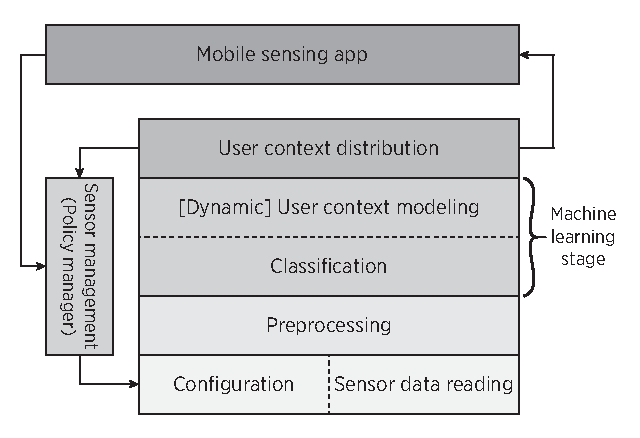
\includegraphics[width=0.5\columnwidth]{generic-middleware-architecture}
  \caption{A generic structure of a middleware following a pure software approach defines explicit modules for selecting and configuring sensor access, and classification and machine learning stages.}
  \label{fig:middleware-software-approach}
\end{figure}



\bibliographystyle{apalike}
\bibliography{../../../resources/references/bibliography}

\end{document}
